175. \begin{figure}[ht!]
\center{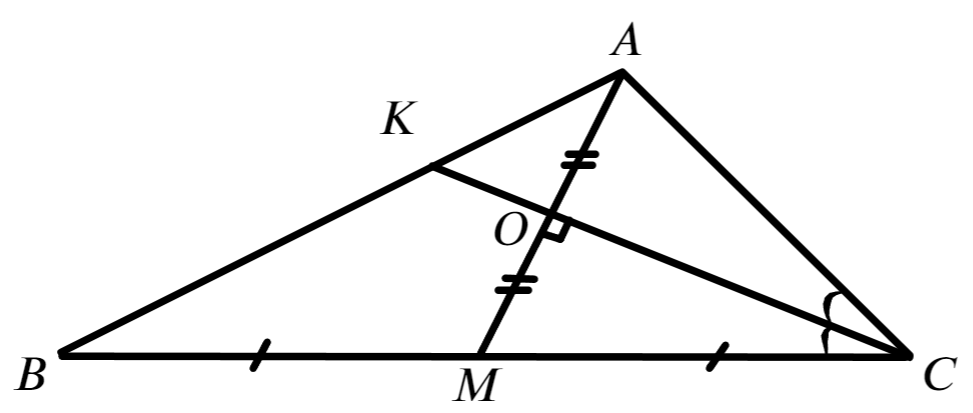
\includegraphics[scale=0.35]{g9-175.png}}
\end{figure}\\
а) Пусть биссектриса $CK$ и медиана $AM$ пересекаются в точке $O.$ В треугольнике $ACM$ биссектриса $CO$ также является высотой, значит он равнобедренный и $CM=AC=4,$ поэтому $BC=2CM=8.$ По теореме об основании биссектрисы имеем соотношение $\cfrac{AK}{KB}=\cfrac{AC}{BC}=\cfrac{4}{8}=\cfrac{1}{2},$ откуда $AK=\cfrac{1}{3}AB=\cfrac{1}{3}\cdot6=2.$\\
б) Так как напротив большей стороны лежит больший угол, необходимо найти $\angle A.$ Запишем теорему косинусов: $BC^2=AB^2+AC^2-2\cdot AB\cdot AC\cdot \cos(\angle A),\ 64=36+16-2\cdot6\cdot4\cdot \cos(\angle A),$ откуда $\cos(\angle A)=-\cfrac{1}{4}.$\\
в) Найдём по формуле для медианы $AM:\ AM=\cfrac{\sqrt{2AB^2+2AC^2-BC^2}}{2}=\cfrac{\sqrt{72+32-64}}{2}=\sqrt{10}.$ По теореме об отрезках хорд для описанной вокруг треугольника $ABC$ окружности получим равенство $BM\cdot MC= AM\cdot MT,\ 4\cdot4=\sqrt{10}\cdot MT$ откуда $MT=\cfrac{16}{\sqrt{10}}.$ Таким образом,
$AT=AM+MT=\sqrt{10}+\cfrac{16}{\sqrt{10}}=\cfrac{26}{\sqrt{10}}=\cfrac{13\sqrt{10}}{5}.$\\
